\section{Qualitative Analysis\label{sec:sota.quali}}

This section contains the results of our literature review.
First, it synthesizes the analyses into a reference architecture and a taxonomy for \glspl{fids}, which help structure the field.
Then, it goes over a comparison of the selected works to answer \Cref{rq:sota.components} on the components of \glspl{fids} and their impact on performance.


\subsection{Structuring the Literature\label{sec:sota.quali.structure}}

The qualitative (\Cref{sec:sota.quali}) and quantitative (\Cref{sec:sota.quanti}) analyzes provide results that we synthesize hereafter in a reference architecture and a taxonomy.
The reference architecture presents the components of \glspl{fids} and their interactions, while the taxonomy provides comparison criteria for the selected works.

We build the taxonomy upon different existing ones related to \gls{cids}
\cite{vasilomanolakis_TaxonomySurveyCollaborative_2015,zhou_surveycoordinatedattacks_2010}, \gls{ml}--based intrusion detection~\cite{dacosta_InternetThingssurvey_2019}, and
\gls{fl} \cite{aledhari_FederatedLearningSurvey_2020,lyu_ThreatsFederatedLearning_2020,mothukuri_surveysecurityprivacy_2021}.
First, we extract classes relevant to the domain
of \gls{fids}, before filtering out irrelevant ones by validating the taxonomy against the reference architecture (\Cref{fig:sota.archi}).
The latter displays both the operation and
the design of the system.
By confronting the taxonomy and the architecture, we ensure that each item
of the taxonomy is related to a component of the architecture, and \emph{vice versa}.
Then, we add any commonalities between the selected works that are not already represented in the previous taxonomies.
This identifies new criteria on which to compare the selected works.


\subsubsection{Reference Architecture\label{sec:sota.discuss.synthesis.archi}}

\begin{figure*}
  \centering
  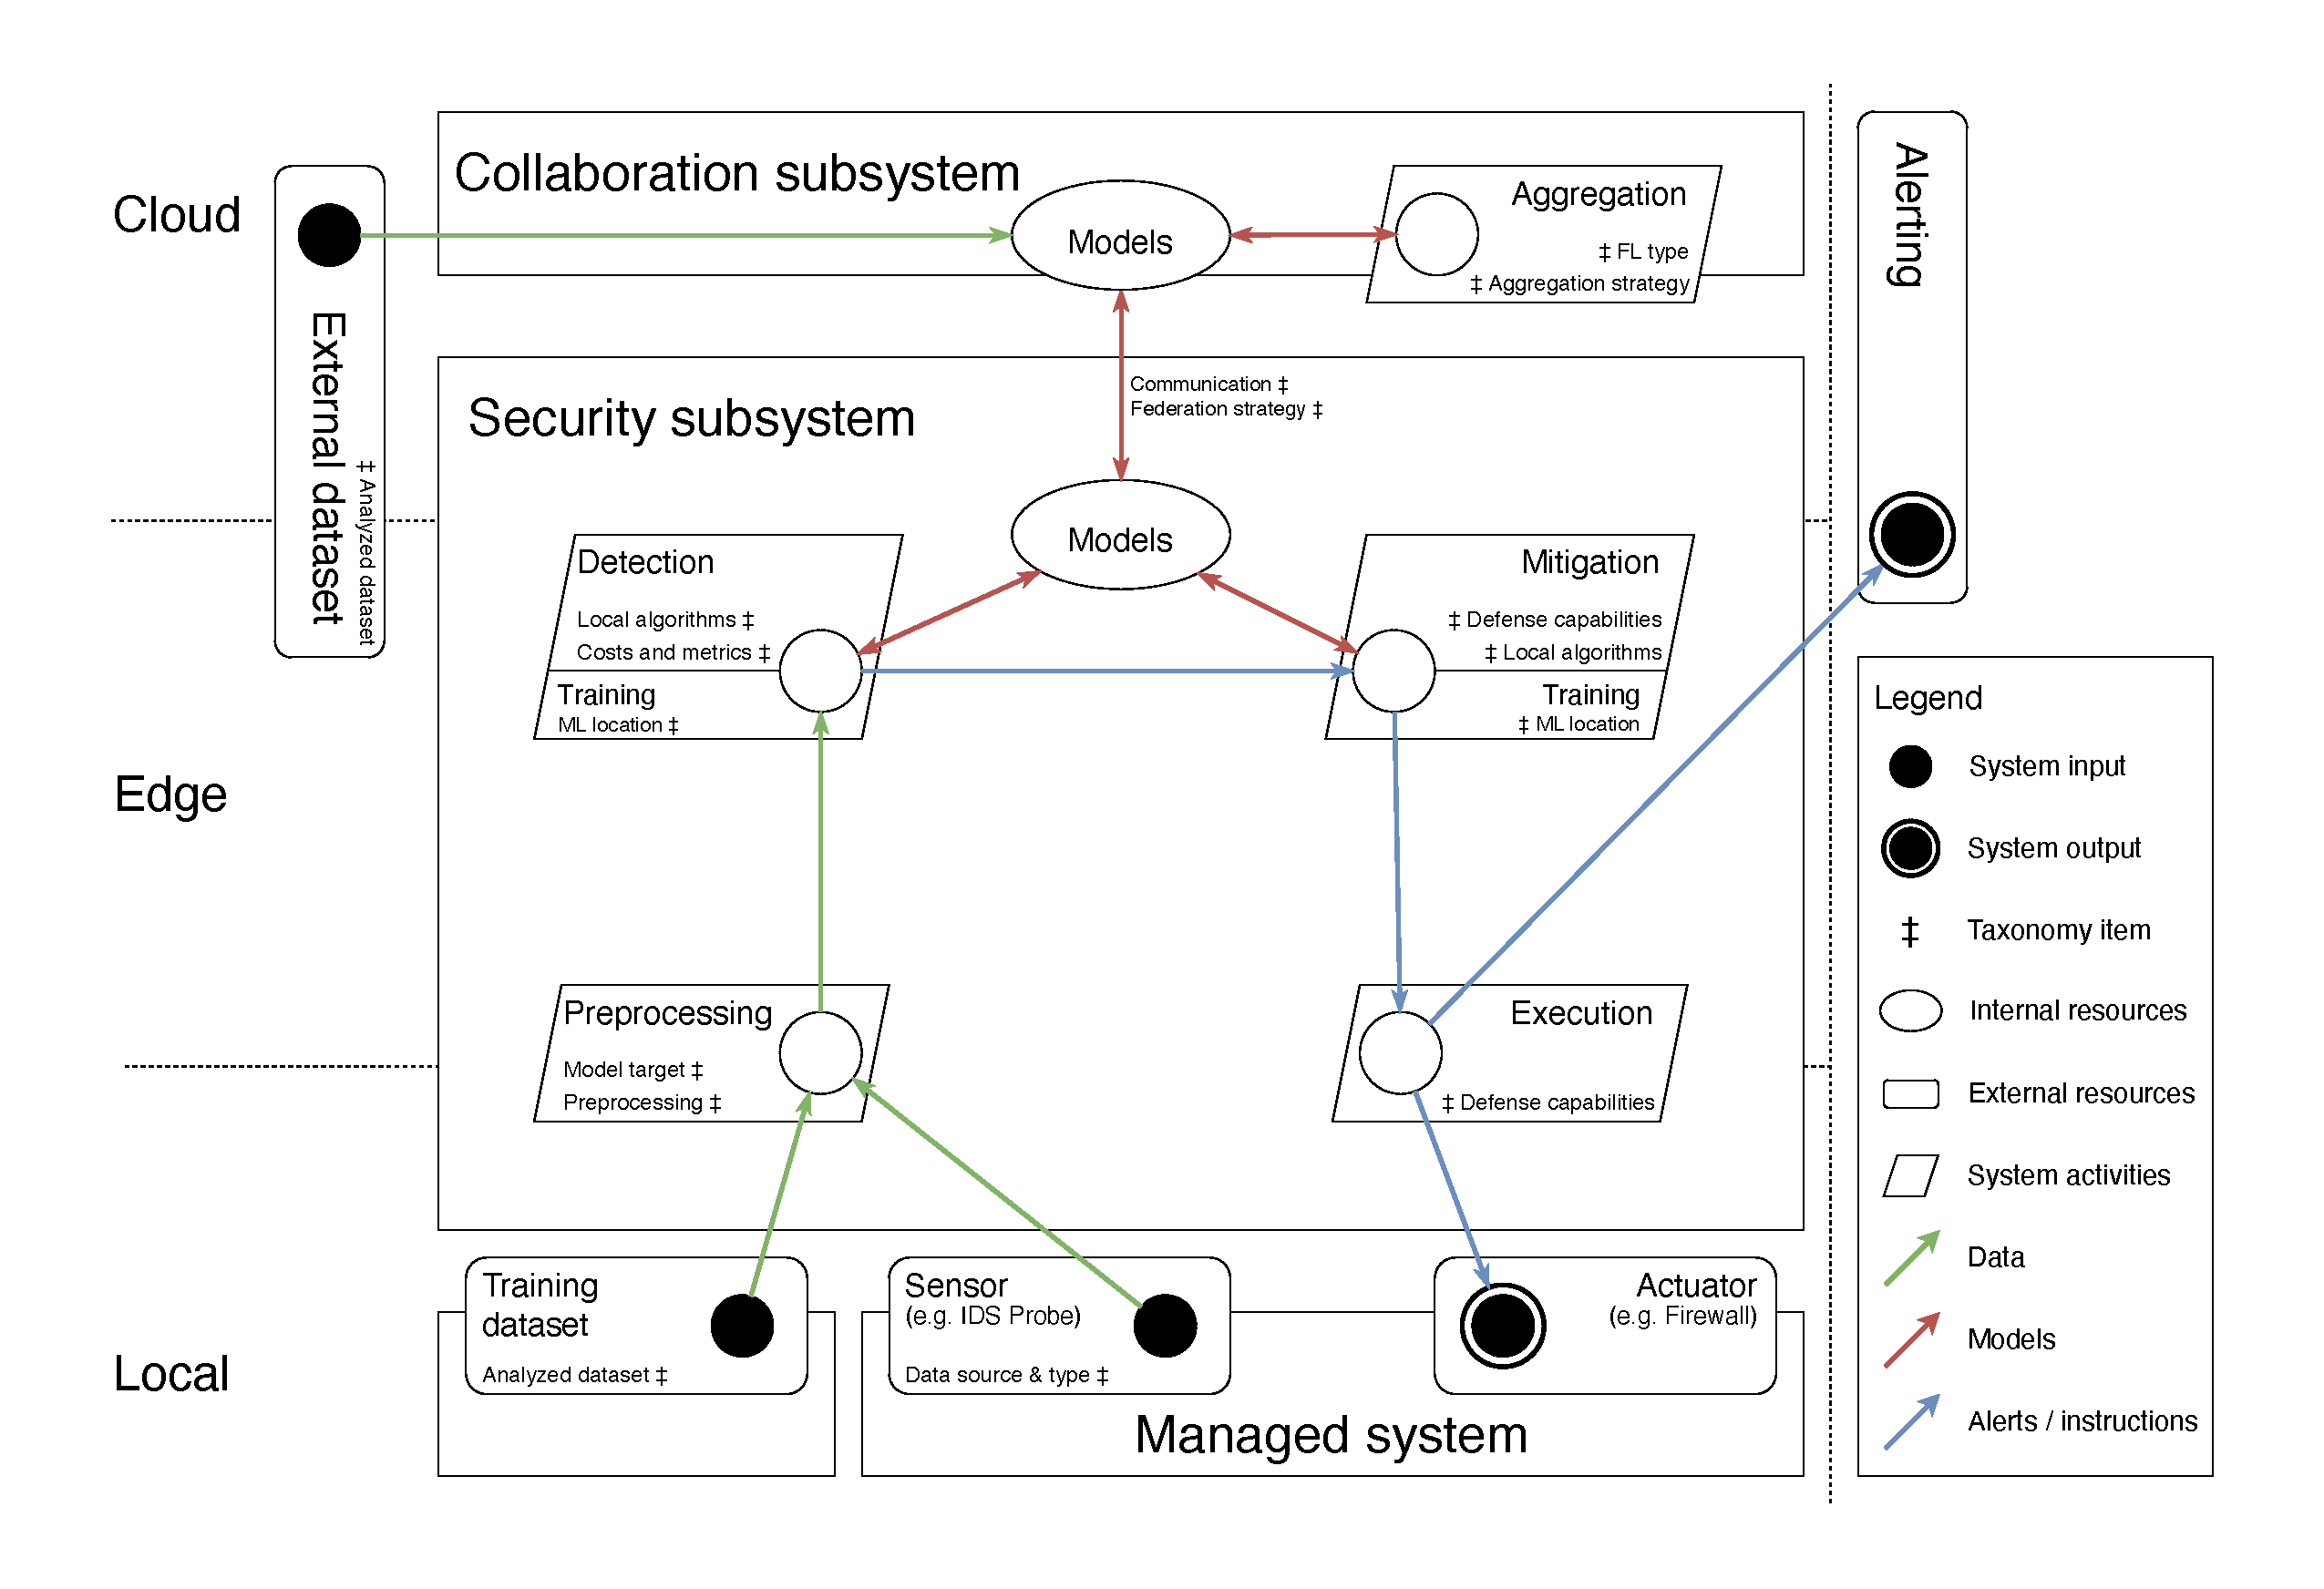
\includegraphics[width=.95\textwidth]{figures/architecture.drawio.pdf}
  \caption{The proposed reference architecture for \glspl{fids}---Figure from \textcite{lavaur_EvolutionFederatedLearningbased_2022} \copyright~IEEE 2022.}
  \label{fig:sota.archi}
\end{figure*}

This section presents the reference architecture synthesized from the selected works, as depicted in \Cref{fig:sota.archi}.
It can be divided in three parts:
\begin{itemize}
  \item The \emph{Managed system} represents the monitored system, \eg, \gls{it} network, industrial devices, or health-monitoring wearables.
  As noticed in \Cref{sec:sota.quali.data}, collected data can either concern system or environment behavior.
  The former relates to information generated by the systems, \eg, network traces or resource consumption.
  The latter refers to what the monitored system operates on, \eg, health metrics for medical devices of temperature and atmospheric pressure for building management systems.
  
  \item The \emph{Security subsystem} is the core of the architecture.
  It contains all the system's activities, from model training to detection and counter-measures deployment.
  Depending on the objectives and constraints, this subsystem can either be run locally like \cite{pahl_AllEyesYou_2018} or \cite{hei_trustedfeatureaggregator_2020}, on a dedicated edge-device as in \cite{li_DeepFedFederatedDeep_2020}.
  In the case of centralized learning, this entire subsystem runs in the cloud.
  The subsystem is assumed to run a device that embeds enough computing power to perform real-time anomaly detection against \gls{ml} models.
  It is also capable of training its own model based on collected data.

  \item The \emph{Collaboration subsystem} provides the \emph{sharing} feature of the system, essentially model aggregation (\Cref{sec:sota.quali.agg}).
  It also provides optional training from other sources, like online datasets.
\end{itemize}

This architecture has similarities with the principles of autonomic systems, as defined by IBM in 2001~\cite{kephart_visionautonomiccomputing_2003}, referred to as \gls{mape-k}.
Classic autonomic systems are local, and therefore use a database to provide \emph{knowledge}.
In \gls{fids}, \gls{fl} fills this role in the reference architecture, as the knowledge is being shared among all agents through model aggregation.


\subsubsection{Taxonomy for FIDS\label{sec:sota.discuss.synthesis.taxo}}

The taxonomy depicted in \Cref{fig:sota.taxonomy} summaries the core components and specificities of \glspl{fids}, as extracted from the selected works and existing related taxonomies.
Correlations between the taxonomy items and the system's components can be seen in the reference architecture (\Cref{fig:sota.archi}).
It also serves as a framework for the comparisons of the selected works.
Each class represents a building block, for which multiple approaches exist depending on use case and constraints.

\begin{figure}
  \centering
  \resizebox{\textwidth}{!}{

\usetikzlibrary{trees,positioning,shapes,shadows,arrows,arrows.meta,angles,quotes}

\definecolor{yellowfill}{HTML}{FFF2CC}
\definecolor{yellowstroke}{HTML}{D6B656}

\definecolor{grayfill}{HTML}{F5F5F5}
\definecolor{graystroke}{HTML}{666666}

\forestset{
  forked edge'/.style={
    edge={rotate/.option=!parent.grow},
    edge path'={
      (.child anchor)
      -- ++(-\forestoption{fork sep},0)
      |- (!u.parent anchor)
    },
  },
}

\newcommand{\lkbx}[1]{\mbox{#1\strut}}



        \begin{forest}
        forked edges,
        for tree={
            rounded corners,
            grow=east,
            inner ysep=1.2ex, 
            anchor=base west,
            l sep+=3em,
            fork sep=2.5em,
            tier/.option=level,
            where level=0{%
                draw,
                draw=yellowstroke,
                fill=yellowfill,
                inner sep=4ex,
                font=\Large\bfseries,
            }{},
            where level=1{%
                draw,
                draw=graystroke,
                fill=grayfill,
                inner sep=3ex,
                font=\Large,
            }{},
            where level=2{%
                draw,
                draw=graystroke,
                fill=grayfill,
                inner sep=3ex,
                font=\large,
            }{},
        },
        parent anchor=east,
        [{Taxonomy of FIDS}
            [Experimentation
                [12. \lkbx{\fullcref{sec:sota.quali.metrics}}
                    [Execution
                        [Performance (\eg accuracy)]
                        [Latency]
                    ]
                    [Federation
                        [Communication]
                        [Aggregation]
                    ]
                    [Training
                        [Resources (\eg hardware)]
                        [Time (\eg convergence)]
                    ]
                ]
                [11. \lkbx{\fullcref{sec:sota.quali.dataset}}
                    [Public / Known]
                    [Published but custom]
                    [Unpublished (as of now)]
                ]
            ]
            [Aggregation
                [10. \lkbx{\fullcref{sec:sota.quali.target}}
                    [By-device]
                    [Personalized model
                        [By-class]
                        [By performance]                
                    ]
                    [Generic model]
                ]
                [9. \lkbx{\fullcref{sec:sota.quali.agg}}
                    [Parameter aggregation (\eg FedAvg)]
                    [Weighted algorithms]
                    [MPC-based aggregation]
                ]
                [8. \lkbx{\fullcref{sec:sota.quali.type}}
                    [Horizontal Federated Learning]
                    [Vertical Federated Learning]
                    [Federated Transfer Learning]
                ]
            ]
            [Federation
                [7. \lkbx{\fullcref{sec:sota.quali.comm}}
                    [Encryption]
                    [Overhead reduction]
                ]
                [6. \lkbx{\fullcref{sec:sota.quali.fed}}
                    [Client selection]
                    [Reputation]
                    [Architecture (\eg P2P)]
                ]
            ]
            [Local operation
                [5. \lkbx{\fullcref{sec:sota.quali.defense}}
                    [Network reconfiguration (\eg SDN)]
                    [On-device counter-measures]
                ]
                [4. \lkbx{\fullcref{sec:sota.quali.alg}}
                    [Supervised ML
                        [Classification]
                        [Regression]
                    ]
                    [Unsupervised ML
                        [Clustering]
                        [Dimensionality reduction]
                        [Outlier detection]
                    ]
                    % [Detection method
                    %     [Anomaly-based]
                    %     [Signature-based]
                    %     [Specification-based]
                    %     [Hybrid]
                    % ]
                ]
                [3. \lkbx{\fullcref{sec:sota.quali.location}}
                    [On device]
                    [On gateway]
                    [Dedicated device]
                    [On server]
                ]
            ]
            [Data
                [2. \lkbx{\fullcref{sec:sota.quali.preprocess}}
                    [Feature selection]
                    [Feature extraction]
                    [Dimensionality reduction]
                ]
                [1. \lkbx{\fullcref{sec:sota.quali.data}}
                    [Source
                        [Communication]
                        [Usage]
                    ]
                    [Distribution
                        [IID]
                        [Non-IID]
                    ]
                ]
            ]
        ]
    \end{forest}
}
  \caption{
    Proposed taxonomy for FIDS---Figure from \textcite{lavaur_EvolutionFederatedLearningbased_2022} \copyright~IEEE 2022.
    \label{fig:sota.taxonomy}
  }
\end{figure}


The proposed taxonomy contains 12 classes describing the selected works that span over five main aspects:
\begin{itemize}
  \item Two classes cover the topic of \textbf{Data}: \emph{Data source \& type} and \emph{Preprocessing}.
  It defines the type of data considered, how it is collected, and the preprocessing strategies that are used.
  
  \item \textbf{Local operation} is represented by 3 classes: \emph{ML location}, \emph{Local algorithms}, and \emph{Defense capabilities}.
  It describes the detection and mitigation strategies, how models are built and trained, and where the computing resources are located.
  
  \item The \textbf{Federation} aspect is covered by 2 classes: \emph{Federation strategy} and \emph{Communication}.
  They refer to the communication between the agents and the server, and how data sharing is organized.
  
  \item \textbf{Aggregation} is also covered by 3 classes: \emph{FL type}, \emph{Aggregation strategy}, and \emph{Model target}.
  It describes the type of \gls{fl} used, how the models are merged, in accordance with the objectives of the system.
  
  \item Finally, 2 classes define the \textbf{Experimentation} topic: \emph{Analyzed dataset} and \emph{Costs and metrics}.
  This meta-category does not relate to the proposed solution, but to how the experiments are performed.
\end{itemize}



\subsection{Federated Learning for Intrusion Detection\label{sec:sota.quali.fids}}

This section reviews the selected literature.
Using the taxonomy as a reference, it details and compares the selected works.
\Cref{tbl:sota.comp} summarizes the information and helps identify differences between the works.
It gives partial answers to research questions about the components of \glspl{fids} and how to measure their impact on performance (\Cref{rq:sota.components,rq:sota.metrics}), while \Cref{sec:sota.quali.agg} replies to \Cref{rq:sota.techniques} about federation techniques.


\begin{table}[]
  \centering
  \caption{
    Comparative overview of selected works---approach and objectives (1/2)
    \label{tbl:sota.comp}
  }
  \resizebox{\textwidth}{!}{% LTeX: enabled=false
        
\newcommand*\rotbr[1]{\hbox to1.5em{\hss\rotatebox[origin=br]{-50}{#1}}}
\newcommand*\rotbl[1]{\hbox to1.5em{\hss\rotatebox[origin=tl]{50}{#1}}} % kept to rotate the bottom row if needed
\newcommand*\rotl[1]{\hbox to1em{\hss\rotatebox{90}{#1}}}
\newcommand*\rotb[1]{#1}
\newcommand*\yes{\CIRCLE}
\newcommand*\partly{\LEFTcircle}
\newcommand*\nop{\Circle}

%\renewcommand{\arraystretch}{2} % add vertical space
% define a tabular environment that has an arraystretch value of 1, allowing
% the main table to have another value.
\newenvironment{1xtabular}[1][1]{%
    \renewcommand*{\arraystretch}{1}%
    \tabular%
}{%
    \endtabular
}

\newenvironment{2xtabular}[1][1]{%
    \renewcommand*{\arraystretch}{2.5}%
    \tabular%
}{%
    \endtabular%
}

\newcommand{\wcell}[1]{\begin{1xtabular}[c]{@{}l@{}}#1\end{1xtabular}}

\begin{threeparttable}

    % WHEN PASTING THE TABLE FROM TABLEGENERATOR:
    % - add the @{} when needed to collapse columns 
    % - replace the in-table tabular environment by `1tabular`
    \begin{2xtabular}{@{}llc@{}c@{}c@{}c@{}cc@{}c@{}c@{}c@{}cc@{}c@{}c@{}c@{}cc@{}clll@{}}
        \toprule
        \multicolumn{1}{c}{} & \multicolumn{1}{c}{Ref}                                                          & \rotbr{Internet of Things} & \rotbr{Information Technologies} & \rotbr{Cyber Physical Systems} & \rotbr{Autonomous Vehicles} & \rotbr{Satellite-terrestrial networks} & \rotbr{Horizontal FL} & \rotbr{Vertical FL} & \rotbr{Federated Transfer Learning} & \rotbr{Federated MTL} & \rotbr{Federated Mimic Learning} & \rotbr{Online learning} & \rotbr{Supervised}  & \rotbr{Semi-supervised}   & \rotbr{Unsupervised}  & \rotbr{Personalized models} & \rotbr{Network-based} & \rotbr{Usage-based} & \multicolumn{1}{c}{Training location}       & \multicolumn{1}{c}{Data type}                         & \multicolumn{1}{c}{Strengths}                                                      \\ \midrule   
        2018                 & \mbox{\textcite{pahl_AllEyesYou_2018}\strut}                                     & \yes                       & \nop                             & \nop                           & \nop                        & \nop                                   & \yes                  & \nop                & \nop                                & \nop                  & \nop                             & \yes                    & \nop                & \nop                      & \yes                  & \yes                        & \yes                  & \nop                & Device                                      & \wcell{Abstracted network\\ traffic (middleware)}     & \wcell{relatively lightweight,\\ online, no labels}                                \\            
        2019                 & \mbox{\textcite{rathore_BlockSecIoTNetBlockchainbaseddecentralized_2019}\strut}  & \nop                       & \yes                             & \nop                           & \nop                        & \nop                                   & \yes                  & \nop                & \nop                                & \nop                  & \nop                             & \nop                    & \yes                & \nop                      & \nop                  & \yes                        & \yes                  & \nop                & \wcell{Edge-controller\\ (SDN)}             & Network traffic (SDN)                                 & \wcell{offers mitigation,\\ decentralized}                                         \\            
        2019                 & \mbox{\textcite{schneble_Attackdetectionusing_2019}\strut}                       & \yes                       & \nop                             & \nop                           & \nop                        & \nop                                   & \yes                  & \nop                & \nop                                & \nop                  & \nop                             & \yes                    & \nop                & \nop                      & \yes                  & \yes                        & \yes                  & \nop                & Gateway                                     & \wcell{IoT network\\ traffic (TCPdump)}               & \wcell{online, offers per-class\\ models, no labels}                               \\            
        2019                 & \mbox{\textcite{nguyen_DIoTFederatedSelflearning_2019}\strut}                    & \nop                       & \yes                             & \nop                           & \nop                        & \nop                                   & \nop                  & \nop                & \nop                                & \yes                  & \nop                             & \nop                    & \yes                & \nop                      & \nop                  & \yes                        & \yes                  & \nop                & Gateway                                     & \wcell{Encrypted network\\ traffic (CICFlowMeter)}    & versatile (multi-task)                                                             \\            
        2019                 & \mbox{\textcite{zhao_MultiTaskNetworkAnomaly_2019}\strut}                        & \nop                       & \nop                             & \yes                           & \nop                        & \nop                                   & \yes                  & \nop                & \nop                                & \nop                  & \nop                             & \yes                    & \nop                & \nop                      & \yes                  & \nop                        & \nop                  & \yes                & Gateway                                     & Healthcare sensor values                              & high adaptability, no labels                                                       \\            
        2019                 & \mbox{\textcite{cetin_FederatedWirelessNetwork_2019}\strut}                      & \nop                       & \yes                             & \nop                           & \nop                        & \nop                                   & \yes                  & \nop                & \nop                                & \nop                  & \nop                             & \nop                    & \yes                & \nop                      & \nop                  & \nop                        & \yes                  & \nop                & Gateway                                     & Network traffic (WIFI)                                & --                                                                                 \\            
        2020                 & \mbox{\textcite{li_DeepFedFederatedDeep_2020}\strut}                             & \yes                       & \nop                             & \nop                           & \nop                        & \nop                                   & \yes                  & \nop                & \nop                                & \nop                  & \nop                             & \nop                    & \yes                & \nop                      & \nop                  & \nop                        & \nop                  & \yes                & Gateway                                     & \wcell{Air conditioner\\ sensor values}               & offers traceability (blockchain)                                                   \\            
        2020                 & \mbox{\textcite{chen_Networkanomalydetection_2020}\strut}                        & \nop                       & \nop                             & \yes                           & \nop                        & \nop                                   & \yes                  & \nop                & \nop                                & \nop                  & \nop                             & \nop                    & \yes                & \nop                      & \nop                  & \nop                        & \yes                  & \nop                & Gateway                                     & MODBUS traffic                                        & confidentiality (encryption)                                                       \\            
        2020                 & \mbox{\textcite{zhang_BlockchainbasedFederatedLearning_2020}\strut}              & \nop                       & \yes                             & \nop                           & \nop                        & \nop                                   & \yes                  & \nop                & \nop                                & \nop                  & \nop                             & \nop                    & \yes                & \nop                      & \nop                  & \nop                        & \yes                  & \nop                & Device                                      & \wcell{IoT network\\ traffic (TCPdump)}               & --                                                                                 \\            
        2020                 & \mbox{\textcite{fan_IoTDefenderFederatedTransfer_2020}\strut}                    & \nop                       & \yes                             & \nop                           & \nop                        & \nop                                   & \yes                  & \nop                & \nop                                & \nop                  & \nop                             & \nop                    & \nop                & \nop                      & \yes                  & \nop                        & \yes                  & \nop                & Gateway                                     & \wcell{IoT network\\ traffic (TCPdump)}               & no labels                                                                          \\            
        2020                 & \mbox{\textcite{rahman_InternetThingsIntrusion_2020}\strut}                      & \nop                       & \yes                             & \nop                           & \nop                        & \nop                                   & \yes                  & \nop                & \nop                                & \nop                  & \nop                             & \nop                    & \yes                & \nop                      & \nop                  & \yes                        & \yes                  & \nop                & Gateway                                     & \wcell{Network traffic\\ (PCAP)}                      & \wcell{segmented (performance-\\based models)}                                     \\            
        2020                 & \mbox{\textcite{sun_IntrusionDetectionSegmented_2020}\strut}                     & \yes                       & \nop                             & \nop                           & \nop                        & \nop                                   & \nop                  & \nop                & \yes                                & \nop                  & \nop                             & \nop                    & \yes                & \nop                      & \nop                  & \yes                        & \yes                  & \nop                & \wcell{Gateway\\ (MEC)}                     & \wcell{IoT network traffic\\ (TCPdump, CICFlowMeter)} & \wcell{knowledge transfer between\\ public and private datasets}                   \\            
        2020                 & \mbox{\textcite{al-athbaal-marri_FederatedMimicLearning_2020}\strut}             & \nop                       & \yes                             & \nop                           & \nop                        & \nop                                   & \nop                  & \nop                & \nop                                & \nop                  & \yes                             & \nop                    & \yes                & \nop                      & \nop                  & \nop                        & \yes                  & \nop                & Gateway                                     & \wcell{Network traffic\\ (TCPdump)}                   & \wcell{enhanced privacy\\ (mimic learning)}                                        \\            
        2020                 & \mbox{\textcite{kim_CollaborativeAnomalyDetection_2020}\strut}                   & \nop                       & \yes                             & \nop                           & \nop                        & \nop                                   & \yes                  & \nop                & \nop                                & \nop                  & \nop                             & \nop                    & \yes                & \nop                      & \nop                  & \nop                        & \yes                  & \nop                & Gateway                                     & \wcell{Network traffic\\ (TCPdump)}                   & --                                                                                 \\            
        2020                 & \mbox{\textcite{qin_LineSpeedScalableIntrusion_2020a}\strut}                     & \nop                       & \yes                             & \nop                           & \nop                        & \nop                                   & \yes                  & \nop                & \nop                                & \nop                  & \nop                             & \nop                    & \yes                & \nop                      & \nop                  & \yes                        & \yes                  & \nop                & \wcell{Gateway\\ (SDN)}                     & Network traffic (SDN)                                 & \wcell{very lightweight,\\ line-speed classification,\\ P4 language compatible}    \\            
        2020                 & \mbox{\textcite{chen_IntrusionDetectionWireless_2020}\strut}                     & \nop                       & \yes                             & \nop                           & \nop                        & \nop                                   & \yes                  & \nop                & \nop                                & \nop                  & \nop                             & \nop                    & \yes                & \nop                      & \nop                  & \nop                        & \yes                  & \nop                & Gateway                                     & \wcell{Network traffic\\ (CICFlowMeter)}              & \wcell{robust to poisoning,\\ scalable}                                            \\            
        2020                 & \mbox{\textcite{hei_trustedfeatureaggregator_2020}\strut}                        & \nop                       & \yes                             & \nop                           & \nop                        & \nop                                   & \yes                  & \nop                & \nop                                & \nop                  & \nop                             & \yes                    & \nop                & \yes                      & \nop                  & \nop                        & \yes                  & \nop                & Device                                      & \wcell{Network traffic\\ (TCPdump)}                   & \wcell{online, offers traceability\\ (blockchain)}                                 \\            
        2020                 & \mbox{\textcite{li_DistributedNetworkIntrusion_2020}\strut}                      & \nop                       & \yes                             & \nop                           & \nop                        & \yes                                   & \yes                  & \nop                & \nop                                & \nop                  & \nop                             & \nop                    & \yes                & \nop                      & \nop                  & \nop                        & \yes                  & \nop                & Gateway                                     & \wcell{Network traffic (PCAP,\\ CICFlowMeter, Argus)} & \wcell{relatively lightweight,\\ confidentiality (encryption)}                     \\            
        2021                 & \mbox{\textcite{liu_BlockchainFederatedLearning_2021}\strut}                     & \yes                       & \nop                             & \nop                           & \nop                        & \nop                                   & \yes                  & \nop                & \nop                                & \nop                  & \nop                             & \nop                    & \yes                & \nop                      & \nop                  & \nop                        & \yes                  & \nop                & Gateway                                     & \wcell{IoT network\\ traffic (TCPdump, Argus)}        & zero-days detection                                                                \\            
        2021                 & \mbox{\textcite{popoola_FederatedDeepLearning_2021}\strut}                       & \nop                       & \yes                             & \nop                           & \nop                        & \nop                                   & \yes                  & \nop                & \nop                                & \nop                  & \nop                             & \nop                    & \yes                & \nop                      & \nop                  & \yes                        & \yes                  & \nop                & Device                                      & \wcell{Network traffic\\ (TCPdump)}                   & relatively lightweight                                                             \\            
        2021                 & \mbox{\textcite{qin_FederatedLearningBasedNetwork_2021}\strut}                   & \nop                       & \nop                             & \nop                           & \yes                        & \nop                                   & \yes                  & \nop                & \nop                                & \nop                  & \nop                             & \nop                    & \yes                & \nop                      & \nop                  & \nop                        & \yes                  & \nop                & Device                                      & \wcell{Network traffic\\ (TCPdump)}                   & decentralized                                                                      \\            
        2021                 & \mbox{\textcite{sun_AdaptiveIntrusionDetection_2021}\strut}                      & \nop                       & \yes                             & \nop                           & \nop                        & \nop                                   & \yes                  & \nop                & \nop                                & \nop                  & \nop                             & \nop                    & \yes                & \nop                      & \nop                  & \yes                        & \yes                  & \nop                & Gateway                                     & \wcell{Network traffic\\ (PCAP)}                      & \wcell{segmented (performance-\\based models)}                                     \\ \midrule   
        \multicolumn{1}{c}{} & \multicolumn{1}{c}{}                                                             & \multicolumn{5}{c}{Use case}                                                                                                                                          & \multicolumn{5}{c}{FL type}                                                                                                                  & \multicolumn{5}{c}{Training}                                                                                                    & \multicolumn{2}{c}{Approach}                & \multicolumn{1}{c}{}                        & \multicolumn{1}{c}{}                                  & \multicolumn{1}{c}{}                                                               \\ \bottomrule
    \end{2xtabular}
\end{threeparttable}
        
}
\end{table}

\begin{table}[]
  \centering
  \caption{
    Comparative overview of selected works---algorithms and performance (2/2)
    \label{tbl:selected.perf}
  }
  \resizebox{\textwidth}{!}{% LTeX: enabled=false
        
\newcommand*\rotbr[1]{\hbox to1.5em{\hss\rotatebox[origin=br]{-50}{#1}}}
\newcommand*\rotbl[1]{\hbox to1.5em{\hss\rotatebox[origin=tl]{50}{#1}}} % kept to rotate the bottom row if needed
\newcommand*\rotl[1]{\hbox to1em{\hss\rotatebox{90}{#1}}}
\newcommand*\rotb[1]{#1}
\newcommand*\yes{\CIRCLE}
\newcommand*\partly{\LEFTcircle}
\newcommand*\nop{\Circle}

%\renewcommand{\arraystretch}{2} % add vertical space
% define a tabular environment that has an arraystretch value of 1, allowing
% the main table to have another value.
\newenvironment{1xtabular}[1][1]{%
    \renewcommand*{\arraystretch}{1}%
    \tabular%
}{%
    \endtabular
}

\newenvironment{2xtabular}[1][1]{%
    \renewcommand*{\arraystretch}{2}%
    \tabular%
}{%
    \endtabular%
}

\newcommand{\wcell}[1]{\begin{1xtabular}[c]{@{}l@{}}#1\end{1xtabular}}

\begin{threeparttable}

    % WHEN PASTING THE TABLE FROM TABLEGENERATOR:
    % - add the @{} when needed to collapse columns 
    % - replace the in-table tabular environment by `1tabular`
    \begin{2xtabular}{@{}llllrrrrrrl@{}}
        \toprule
        \multicolumn{1}{c}{} & \multicolumn{1}{c}{Ref}                                                          & \multicolumn{1}{c}{Local Algorithm}                                               & \multicolumn{1}{c}{Federation Algorithm} & \multicolumn{1}{c}{Accuracy} & \multicolumn{1}{c}{Precision} & \multicolumn{1}{c}{Recall} & \multicolumn{1}{c}{Fall-out} & \multicolumn{1}{c}{F-Score} & \multicolumn{1}{c}{\(K\) \(^a\)}  & \multicolumn{1}{c}{Dataset}                                                                                                                                                                                                                       \\ \midrule
        2018                 & \mbox{\textcite{pahl_AllEyesYou_2018}\strut}                                     & \wcell{BIRCH\\ K-means}                                                           & Parameter addition                       & 0.9900                       & --                            & 0.9600                     & 0.0020                       & --                          & 7                                 & Generated                                                                                                                                                                                                                                         \\
        2019                 & \mbox{\textcite{rathore_BlockSecIoTNetBlockchainbaseddecentralized_2019}\strut}  & ANN                                                                               & Vector concatenation                     & \(\ddagger\) 0.9100          & \(\ddagger\) 0.9100           & \(\ddagger\) 0.9100        & --                           & \(\ddagger\) 0.9100         & 15                                & NSL-KDD \mbox{\cite{tavallaee_detailedanalysisKDD_2009}\strut}                                                                                                                                                                                    \\
        2019                 & \mbox{\textcite{schneble_Attackdetectionusing_2019}\strut}                       & MLP                                                                               & Weight and biases average                & 0.9930                       & --                            & --                         & --                           & --                          & 64                                & MIMIC \mbox{\cite{johnson_MIMICIIIfreelyaccessible_2016}\strut}                                                                                                                                                                                   \\
        2019                 & \mbox{\textcite{nguyen_DIoTFederatedSelflearning_2019}\strut}                    & GRU                                                                               & FedAvg                                   & --                           & --                            & 0.9543                     & 0                            & --                          & 15                                & Generated                                                                                                                                                                                                                                         \\
        2019                 & \mbox{\textcite{zhao_MultiTaskNetworkAnomaly_2019}\strut}                        & FC (shared layers) \(\rightarrow\) FC                                             & Weight and biases average                & \(\ast\) 0.9797              & \(\ast\) 0.9634               & \(\ast\) 0.9681            & --                           & --                          & --                                & \wcell{CICIDS2017~\mbox{\cite{sharafaldin_GeneratingNewIntrusion_2018}\strut}\\ ISCXVPN2016~\mbox{\cite{draper-gil_CharacterizationEncryptedVPN_2016}\strut}\\ ISCXTor2016~\mbox{\cite{habibilashkari_CharacterizationTorTraffic_2017}\strut}}    \\
        2019                 & \mbox{\textcite{cetin_FederatedWirelessNetwork_2019}\strut}                      & SAE                                                                               & FedAvg                                   & --                           & --                            & --                         & --                           & --                          & 933                               & AWID~\mbox{\cite{kolias_IntrusionDetection802_2016}\strut}                                                                                                                                                                                        \\
        2020                 & \mbox{\textcite{li_DeepFedFederatedDeep_2020}\strut}                             & CNN-GRU \(\rightarrow\) MLP                                                       & Homomorphic parameter addition           & 0.9920                       & 0.9885                        & 0.9745                     & --                           & 0.9813                      & 7                                 & CPS dataset~\mbox{\cite{morris_IndustrialControlSystem_2014}\strut}                                                                                                                                                                               \\
        2020                 & \mbox{\textcite{chen_Networkanomalydetection_2020}\strut}                        & DAGMM                                                                             & Parameter addition                       & --                           & 0.7447                        & 0.9803                     & --                           & \(\ddagger\) 0.8700         & 2 \(^b\)                          & KDD 99 \mbox{\cite{kddcup99}\strut}                                                                                                                                                                                                               \\
        2020                 & \mbox{\textcite{zhang_BlockchainbasedFederatedLearning_2020}\strut}              & ANN                                                                               & CDW\_FedAvg                              & \(\ast\ddagger\) 0.8900      & \(\ast\ddagger\) 0.8600       & \(\ast\ddagger\) 0.9450    & --                           & \(\ast\ddagger\) 0.8500     & 4                                 & Generated                                                                                                                                                                                                                                         \\
        2020                 & \mbox{\textcite{fan_IoTDefenderFederatedTransfer_2020}\strut}                    & CNN                                                                               & Parameter aggregation                    & \(\ast\) 0.9100              & --                            & \(\ast\ddagger\) 0.9350    & \(\ast\ddagger\) 0.0020      & --                          & 4                                 & \wcell{CICIDS2017~\mbox{\cite{sharafaldin_GeneratingNewIntrusion_2018}\strut}\\ NSL-KDD~\mbox{\cite{tavallaee_detailedanalysisKDD_2009}\strut}\\ Generated}                                                                                       \\
        2020                 & \mbox{\textcite{rahman_InternetThingsIntrusion_2020}\strut}                      & ANN                                                                               & FedAvg                                   & \(\ast\) 0.7731              & --                            & --                         & --                           & --                          & 4                                 & NSL-KDD \mbox{\cite{tavallaee_detailedanalysisKDD_2009}\strut}                                                                                                                                                                                    \\
        2020                 & \mbox{\textcite{sun_IntrusionDetectionSegmented_2020}\strut}                     & CNN                                                                               & Parameter aggregation                    & \(\ast\) 0.8710              & --                            & --                         & --                           & --                          & 20                                & \wcell{LAN-Security\\ Monitoring Project~\mbox{\cite{hideya_LANSecurityMonitoringProject_2018}\strut}}                                                                                                                                            \\
        2020                 & \mbox{\textcite{al-athbaal-marri_FederatedMimicLearning_2020}\strut}             & ANN                                                                               & FedAvg                                   & 0.9812                       & \(\ast\) 0.9900               & \(\ast\) 0.9900            & \(\ast\) 0.1320              & \(\ast\) 0.9900             & 10                                & NSL-KDD \mbox{\cite{tavallaee_detailedanalysisKDD_2009}\strut}                                                                                                                                                                                    \\
        2020                 & \mbox{\textcite{kim_CollaborativeAnomalyDetection_2020}\strut}                   & MLP                                                                               & FedAvg                                   & 0.9712                       & --                            & --                         & --                           & --                          & 4                                 & NSL-KDD \mbox{\cite{tavallaee_detailedanalysisKDD_2009}\strut}                                                                                                                                                                                    \\
        2020                 & \mbox{\textcite{qin_LineSpeedScalableIntrusion_2020a}\strut}                     & BNN                                                                               & SignSGD                                  & \(\ast\) 0.9640              & \(\ast\) 0.9555               & \(\ast\) 0.8645            & --                           & \(\ast\) 0.9055             & 8                                 & \wcell{CICIDS2017~\mbox{\cite{sharafaldin_GeneratingNewIntrusion_2018}\strut}\\ ISCX Botnet 2014~\mbox{\cite{biglarbeigi_effectivefeatureselection_2014}\strut}}                                                                                  \\
        2020                 & \mbox{\textcite{chen_IntrusionDetectionWireless_2020}\strut}                     & GRU-SVM                                                                           & FedAGRU                                  & \(\ast\) 0.9905              & --                            & --                         & \(\ast\) 0.0108              & \(\ast\) 0.9762             & 20                                & \wcell{CICIDS2017~\mbox{\cite{sharafaldin_GeneratingNewIntrusion_2018}\strut}\\ KDD 99 \mbox{\cite{kddcup99}\strut}\\ WSN-DS \mbox{\cite{almomani_WSNDSDatasetIntrusion_2016}\strut}}                                                             \\
        2020                 & \mbox{\textcite{hei_trustedfeatureaggregator_2020}\strut}                        & MLP                                                                               & FedAvg                                   & \(\ast\ddagger\) 0.8950      & \(\ast\ddagger\) 0.9750       & \(\ast\ddagger\) 0.8775    & --                           & \(\ast\ddagger\) 0.9225     & 3                                 & DARPA 1999 \mbox{\cite{haines_1999DARPAIntrusion_2001}\strut}                                                                                                                                                                                     \\
        2020                 & \mbox{\textcite{li_DistributedNetworkIntrusion_2020}\strut}                      & CNN                                                                               & Homomorphic parameter addition           & \(\ast\) 0.8100              &                               &                            & \(\ast\) 0.1900              &                             & 4                                 & Generated                                                                                                                                                                                                                                         \\
        2021                 & \mbox{\textcite{liu_BlockchainFederatedLearning_2021}\strut}                     & MLP                                                                               & Parameter aggregation                    & \(\ddagger\) 0.9600          & 0.9400                        & 0.9500                     & --                           & --                          & 6                                 & KDD 99 \mbox{\cite{kddcup99}\strut}                                                                                                                                                                                                               \\
        2021                 & \mbox{\textcite{popoola_FederatedDeepLearning_2021}\strut}                       & ANN                                                                               & FedAvg                                   & \(\ast\) 0.9939              & \(\ast\) 0.9819               & \(\ast\) 0.9676            & --                           & \(\ast\) 0.9728             & 5                                 & \wcell{Bot-IoT \mbox{\cite{koroniotis_developmentrealisticbotnet_2019}\strut}\\ N-BaIoT \mbox{\cite{meidan_NBaIoTNetworkbasedDetection_2018}\strut}}                                                                                              \\
        2021                 & \mbox{\textcite{qin_FederatedLearningBasedNetwork_2021}\strut}                   & ONLAD \mbox{\cite{tsukada_NeuralNetworkBasedOndevice_2020}\strut} (ELM \(+\) AE)  & FedAvg                                   & 0.7040                       & --                            & --                         & --                           & --                          & 8                                 & NSL-KDD \mbox{\cite{tavallaee_detailedanalysisKDD_2009}\strut}                                                                                                                                                                                    \\
        2021                 & \mbox{\textcite{sun_AdaptiveIntrusionDetection_2021}\strut}                      & CNN                                                                               & Parameter aggregation                    & --                           & --                            & --                         & --                           & \(\ast\) 0.8930             & 20                                & \wcell{LAN-Security\\ Monitoring Project~\mbox{\cite{hideya_LANSecurityMonitoringProject_2018}\strut}}                                                                                                                                            \\ \midrule
        \multicolumn{1}{c}{} & \multicolumn{1}{c}{}                                                             & \multicolumn{1}{c}{}                                                              & \multicolumn{1}{c}{}                     & \multicolumn{5}{c}{Metrics}                                                                                                                            & \multicolumn{1}{c}{}              & \multicolumn{1}{c}{}                                                                                                                                                                                                                              \\ \bottomrule

    \end{2xtabular}

    \begin{tablenotes}
        \item \(\ast\) Value is an average of those provided by the authors.
        \item \(\ddagger\) Value is read from a graph in the article, and may vary a few
        from the exact value.\vspace{2ex}
        \item \(^a\) \(K\) is the highest number of client considered in the experiments.
        \item \(^b\) \textcite{chen_Networkanomalydetection_2020} measure how one client performs, by training one other.
    \end{tablenotes}
    
\end{threeparttable}

    }
\end{table}

\subsubsection{Data Source and Type\label{sec:sota.quali.data}}

Depending on the use case, we observe two main approaches in the selected works.
In the first one~\cite{zhang_BlockchainbasedFederatedLearning_2020,schneble_Attackdetectionusing_2019}, the model is trained on the sensors' values.
While they are not represented in the initial selection, this is closer to \glspl{hids} in operation.
For instance, since~\cite{zhang_BlockchainbasedFederatedLearning_2020} targets medical devices, their values include hearth rate and oxygen saturation.
The opposite strategy operates at a higher level of abstraction, independent of the values, and rather focuses on the communication between devices using network traffic, just like \glspl{nids}.
Most papers \cite{chen_Networkanomalydetection_2020,rathore_BlockSecIoTNetBlockchainbaseddecentralized_2019,nguyen_DIoTFederatedSelflearning_2019,li_DeepFedFederatedDeep_2020,rahman_InternetThingsIntrusion_2020,sun_IntrusionDetectionSegmented_2020,popoola_FederatedDeepLearning_2021a,hei_trustedfeatureaggregator_2020} use similar network features, such as source and destination, local and remote ports, TCP flags, protocol, and packet length.
The authors of \cite{qin_LineSpeedScalableIntrusion_2020a} also target network features but at packet-level, all translated to 1D vectors: IP addresses, layer-4 protocol, ports, and IP packet length as a 120-bit input vector.
\textcite{li_DeepFedFederatedDeep_2020} also explore network-related features in their use case of satellite communications.

These values can be completed with preprocessing (see \Cref{sec:sota.quali.preprocess}) to extract other features from the raw data.
For instance, both \textcite{pahl_AllEyesYou_2018} and \textcite{nguyen_DIoTFederatedSelflearning_2019} analyze the periodicity of packets, which is notably useful for volumetric attack detection.
Furthermore, both work target \gls{iot} devices, which have a sporadic, but periodic and thus more predicable traffic.
In this context, anomaly in the packet-sequence, or in the inter-arrival time might indicate an attack.
While following a similar approach, \gls{ftl} allows the authors of \cite{fan_IoTDefenderFederatedTransfer_2020} to address different features in each client's dataset.

Finally, using a middleware to classify the data, \textcite{pahl_AllEyesYou_2018} can train per-class models with high accuracy.
However, most solutions do not provide such metadata.
Training per-class models requires then a prior classification step, like in \cite{nguyen_DIoTFederatedSelflearning_2019}.

Additionally, even when considering the same data type, use cases introduce significant differences in the available features.
For instance, two systems targeting the communication between devices may encounter different protocols, services, and even communication support.
In the literature, the most common use cases are (sorted by representation): \acrfull{it}, \acrfull{iot}, \acrfull{cps}, and \acrfull{av}.

% The work of \textcite{liu_BlockchainFederatedLearning_2021} is the only representative of the \gls{av} use case, although they do not use an according dataset.
% In fact, they train their model on network traffic, with similar features to \cite{rahman_InternetThingsIntrusion_2020,chen_Networkanomalydetection_2020,rathore_BlockSecIoTNetBlockchainbaseddecentralized_2019,fan_IoTDefenderFederatedTransfer_2020}.
% With also similar features, \textcite{li_DeepFedFederatedDeep_2020b} apply \gls{fids} to the very specific use case of \gls{stin}.

Finally, \cite{chen_Networkanomalydetection_2020}, and partly  \cite{hei_trustedfeatureaggregator_2020}, address data distribution, especially knowing whether data are \gls{iid}.
A non-\gls{iid} data distribution can negatively impact training performance~\cite{Yang2019}.
However, most real-world scenarios generate non-\gls{iid} data, which is a major hurdle for algorithm that require to be trained on live data with non-supervised approaches.

\subsubsection{Preprocessing\label{sec:sota.quali.preprocess}}

\subsubsection{Algorithm location\label{sec:sota.quali.location}}

\subsubsection{Local Algorithm\label{sec:sota.quali.alg}}

\subsubsection{Defense Mechanism\label{sec:sota.quali.defense}}

\subsubsection{Federation Strategy\label{sec:sota.quali.fed}}

\subsubsection{Communication\label{sec:sota.quali.comm}}

\subsubsection{FL Type\label{sec:sota.quali.type}}

\subsubsection{Aggregation Strategy\label{sec:sota.quali.agg}}

\subsubsection{Model Target\label{sec:sota.quali.target}}

\subsubsection{Analysed Dataset\label{sec:sota.quali.dataset}}

\subsubsection{Costs and Metrics\label{sec:sota.quali.metrics}}
